\section{Transportlaget}
Transportlaget ligger i denne protokolsuite mellem applikationslaget og datalinklaget. Grunden til dette er at netværkslaget ikke er relevant i forhold til node til node kommunikation. Transportlaget står for at implementerer flow-og fejlkontrol. Da dette ikke er implementeret i de underliggende lag. Transportlaget står derfor for en pålidelig dataoverførsel over de upålidelige underliggende lag.

\subsection{Protokol Type}
Den simpleste protokol type at implementere er en protokol, hvor data sendes med det samme det modtages fra applikationslaget. Og data sendes op til applikationslaget i det øjeblik transportlaget har modtaget det. Denne protokol type har ingen fejlkontrol eller flow-kontrol. Hvis en pakke går tabt undervejs i forsendelsen f.eks. fordi den er blevet korrupt nede på datalinklaget. Så vil dette aldrig blive opdaget af hverken det modtagende eller det afsendende transportlag. Og data vil derfor være gået tabt. For at opdage dette, kan der implementeres ACK beskeder, der sendes tilbage fra modtageren til afsenderen, og essentielt kvitterer for den modtagende pakke. ACK kan sendes tilbage for hver pakke der bliver modtaget eller der kan køres kumulative ACK's, hvor et ACK kvitterer for flere pakker ad gangen. Der er blevet valgt at implementere stop-and-wait protokollen, der venter med at sende en ny datapakke, til der er modtaget et ACK for den foregående datapakke. Begrundelsen for dette er, at denne protokol giver mulighed for fejltjek uden at der kræves særligt meget for at implementere den, og selve implementeringen danner grundlag for at kunne opgraderes til en anden protokol, hvis behovet opstår. Figur \ref{StopAndWait} viser stop and wait protokollen.
\begin{figure}[h]
\centering
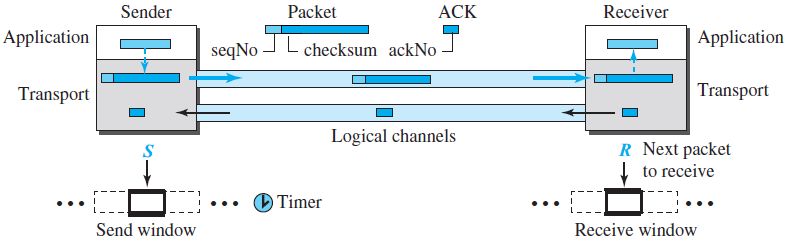
\includegraphics[scale=0.75]{Billeder/StopAndWait.png}
\caption{Stop and wait Protokollen
\label{StopAndWait}}
\end{figure}

\subsubsection{Effektivitet}
Effektiviteten af en stop-and-wait protokol er meget lav, hvis båndbredden på kanalen er høj og udbredelsestiden er meget lang i kanalen. Så hvis der kan sendes mange bits igennem kanalen, og det tager lang tid for dem at nå frem til modtageren, så er stop-and-wait en dårlig ide. I denne implementering kan stop-and-wait dog godt betale sig, da båndbredden kun er på 160bps og udbredelsestiden er lydens hastighed. Dette medvirker at mediet vil virke instantant, og der derfor ikke ville kunne stoppes ekstra bit ind på mediet, mens der ventes på ACK.

\subsection{Flow-kontrol}
Transportlaget implementerer flow kontrol i form af de ACK-beskeder, der sendes efter hver data pakke er modtaget. Idet at implementeringen er en stop-and-wait protokol, skal der ventes på ACK inden det næste data kan sendes. Data kan således kun ankomme i rigtig rækkefølge, da en afsender ikke afsender den næste datapakke før det er blevet bekræftet at pakken er modtaget hos modtageren. Og flow kan også styres ved at lade være med at sende et ACK tilbage på en modtagen pakke, hvis modtageren er for optaget til at pakken kan modtages. Således vil afsenderen gentage afsendelsen af pakken efter timeren udløber og modtageren kan så fortsætte med at nægte modtagelse indtil denne er klar.

\subsection{Fejl-kontrol}
Der er implementeret fejlkontrol i form af sekvensnumre. Afsenderen af data ved hvilket sekvensnummer den forventer at få tilbage på et ACK, og modtageren ved hvilket sekvensnummer den næste modtagne pakke burde have. Et eksempel på, hvordan fejlkontrollen fungerer kan ses i figur \ref{StopAndWaitFlow}.

\begin{figure}[h]
\centering
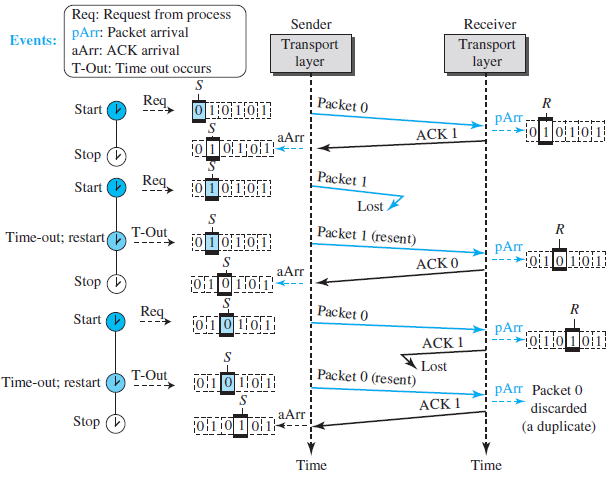
\includegraphics[scale=0.75]{Billeder/StopAndWaitFlow.png}
\caption{flow diagram over Stop-and-Wait protokollen
\label{StopAndWaitFlow}}
\end{figure}

\subsection{Implementering}
Transportlaget er implementeret i en klasse uden nogen hjælpeklasser. Afsender-og modtagerdelen kører i samme tråd, og der skiftes mellem at tjekke for modtagen data, og om der skal afsendes noget data. Hele implementeringen kører i en separat tråd fra det ovenliggende applikationslag og opholder derved ikke applikationslaget. Da transportlaget kører i sin egen tråd, er der sørget for at låse delte attributter, når de tilgås således at der ikke opstår problemer med andre tråde. Hovedfunktion der står for at holde transportlaget kørende er \textit{loop}, der startes op i en tråd af Transportlagets egen constructor.

\subsubsection{Afsending}
Når der afsendes data af transportlaget så er transportlaget inde i funktionen \textit{sendData}. Her oprettes der en frame ud fra den nuværende payload, der ligger klar fra applikationslaget af. Denne frame sendes afsted og funktionen \textit{receiveACK} køres. Inde i funktionen checkes der for om der modtages det korrekte ACK tilbage. Der kører samtidig en timer, der ved udløb resulterer i at transportlaget retransmitterer dataen. Hver gang timeren udløber, inkrementeres der en værdi og når denne værdi er over grænsen for retransmissionsforsøg(der er fastsat i \textit{constants.h}), så stopper transportlaget med at forsøge at sende datapakken afsted, og venter i et tilfældigt stykke tid(med en nedre grænse på 0 og en øvre grænse fastsat i \textit{constants.h}), før den forsøger at sende igen.

\subsubsection{Modtagelse}
Når der modtages data, så er transportlaget inde i funktionen \textit{receiveData}. Her checkes der for om der ligger en modtagen frame klar i bufferen fra datalinklaget. Hvis der gør dette checkes der for om denne frame er en data frame. Hvis ikke det er en dataframe så smides framen væk, men hvis det er en dataframe så checkes der om framen har det sekvensnummer der forventes modtaget. Hvis ikke framen har det, så smides den væk og ellers så sendes der et ACK tilbage, og framen smides i et modtagelsesbuffer som applikationslaget kan tilgå.